
%%%%%%%%%%%%%%%%%%%% file CSMC_MUME_LaTeX_Template.tex %%%%%%%%%%%%%%%%%%%%%
%
% This is the LaTeX source for the instructions to authors using
% the LaTeX document class 'llncs.cls' for contributions to
% the Journal of Creative Music Systems.
% Copyright: http://www.springer.com/lncs       Springer Heidelberg 2006/05/04
%
% It may be used as a template for your own input - copy it
% to a new file with a new name and use it as the basis
% for your article.
%
% NB: the document class 'llncs' has its own and detailed documentation, see
% ftp://ftp.springer.de/data/pubftp/pub/tex/latex/llncs/latex2e/llncsdoc.pdf
%
%%%%%%%%%%%%%%%%%%%%%%%%%%%%%%%%%%%%%%%%%%%%%%%%%%%%%%%%%%%%%%%%%%%

\documentclass[runningheads,a4paper]{llncs}

\usepackage{amssymb}
\setcounter{tocdepth}{3}
\usepackage{graphicx}
\usepackage{url}
\usepackage{apacite}
%added 
\usepackage[inline]{enumitem}    
\usepackage{subcaption}
\usepackage{caption}
\usepackage{threeparttable} %annotations for table
\usepackage{csquotes}


\newcommand{\keywords}[1]{\par\addvspace\baselineskip
\noindent\keywordname\enspace\ignorespaces#1}

\pagestyle{headings}

\begin{document}

\mainmatter  % start of an individual contribution

% first the title is needed
\title{Percussive Sound Generation with Virtual Listeners and Modular Synthesizers}

% a short form should be given in case it is too long for the running head
\titlerunning{Virtual Percussive Sound Generation}

% the name(s) of the author(s) follow(s) next
%
% NB: Chinese authors should write their first names(s) in front of
% their surnames. This ensures that the names appear correctly in
% the running heads and the author index.
%
\author{Amir Salimi \and Abram Hindle}
%
% if the names of the authors are too long for the running head, please use the format: AuthorA et al.
\authorrunning{Amir Salimi and Abram Hindle }

% the affiliations are given next; don't give your e-mail address
% unless you accept that it will be published
\institute{Department of Computing Science\\ University of Alberta \\ \email{asalimi@ualberta.ca}}

%
% NB: a more complex sample for affiliations and the mapping to the
% corresponding authors can be found in the file "llncs.dem"
% (search for the string "\mainmatter" where a contribution starts).
% "llncs.dem" accompanies the document class "llncs.cls".
%

\maketitle

\begin{abstract}
Digital sound artists often require a variety of percussive samples for their music. For more than two decades research involving digital synthesis, heuristic search, and neural networks has been used for the generation of novel sounds. Our goal is to generate one-shot percussive samples by leveraging modern AI technologies alongside scalable signal generation methods. We centered our approach around the combination of two central components: \begin {enumerate*} [label=(\roman*)] \item a \emph{virtual ear} capable of evaluating the proximity of unheard sounds to  and \item a dynamic \emph{virtual synthesizer} with a rich set of tractable parameters\end{enumerate*}. We present a generative pipeline that utilizes robust digital signal processing methods guided by supervised learning towards the generation of one-shot percussive sounds. We present our findings and measurements of the various approaches taken. Advantages, shortcomings and practicality of the employed methodologies are demonstrated. We share our curated dataset of sounds and codebase\footnote{\url{https://github.com/imilas/Synths_Stacks_Search}} which can be used for its further expansion.
\keywords{Automatic Synthesizer design. Machine Listening. Sound Analysis. Novelty and Originality}
\end{abstract}

\section{Preamble}
\subsection{Drums and Percussion}
Drums are a subcategory of percussive instruments. Drum sounds such as kick and snare are two of the most universally recognized examples of percussion~\cite{barry2005drum}. Almost any object which is struck to produce noise can be referred to as a drum~\cite{latham2002oxford}. The term \enquote{Percussion} often encompasses all drums and may include the additional instruments which may be rubbed, plucked, blown, etc; A more strict definition of percussion can be used interchangeably with drums~\cite{latham2002oxford}. We adapt this strict definition for this work as our concern is not the delineation between the two overlapping concepts, but with extraction and creation of novel sounds with characteristics shared between the two. As a result, we often use the terms \enquote{drum} and \enquote{percussion} interchangeably.

\subsection{Motivation and Goals}
Digital recordings of novel, one-shot\footnote{A single hit on the drum that captures its capabilities} drum sounds are not easy or cheap to find. Our goal here is to create a new, virtual source of novel drum sounds, which could then be used in electronic music compositions.

By relying on recordings of \textit{real life} drum sounds, we are limited by what instruments exist in the real world and whether or not we have access to clean, one-shot recordings. Our hypothesis is that the virtualization of sound generation can alleviate these material limitations. 

\subsection{What Solution Do We Propose?}
To virtually create novel drum sounds, we need a generative source; One that produces audio based on some instructions. We also need a method of evaluation to help us determine which sounds resemble drums and are worth keeping. We also would like to know what instructions caused our audio source to make the sounds we liked. In short, our approach requires effective \textit{generation} and \textit{evaluation} of sounds. 
\subsection{How Can a Computer Make Sounds?}
Sounds are transmitted via waveforms. Your computer can emulate the physical characteristics of basic waveforms by evaluating the output of periodic functions such as sines and cosines. Evaluation of basic periodic functions is the simplest form of software audio generation~\cite{mitchell2009basicsynthChap5}.
This generative system is called an \textit{oscillator} and its output is a waveform which can be sent to your computer's digital-to-analog conversion system to create an audible signal. The combination and modification of these pure tones are the building blocks of digital signal processing (DSP).

\begin{figure*}[h]
\label{fig_example_sine}
\centering
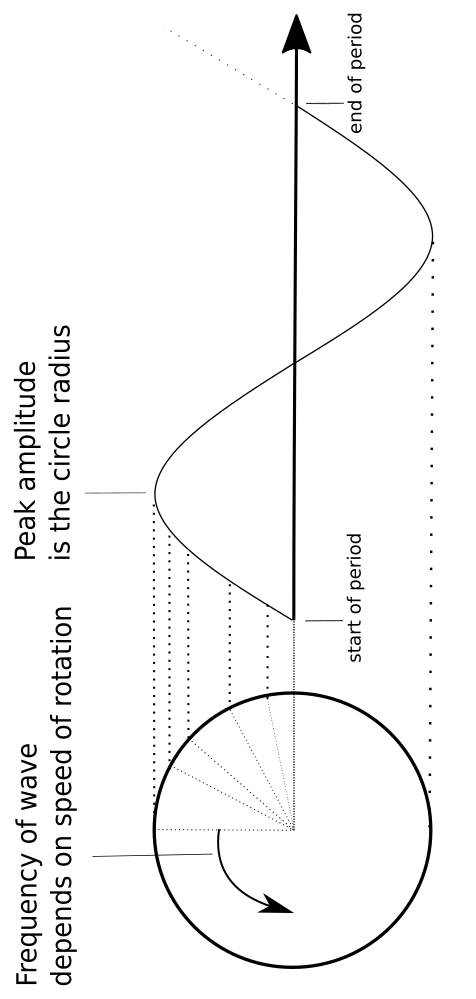
\includegraphics[width=0.45\linewidth,angle =-90 ]{images/periodic_function.png}
\caption{A computer can simulate waveforms by utilizing periodic functions. Digital waveforms are discrete approximations of analogue waves. \cite{mitchell2009basicsynthChap5} }
\end{figure*}


 Most organic sounds---sounds from the natural environment, and its flora and fauna---are much more complex than the output of a single oscillator. However, with careful programming, DSP techniques can be used to replicate almost any sound, which is why they have powered commercial digital synthesizers for over half a century \cite{jenkins2019analog}. Another advantage to using DSP for sound generation is that the synthesizers we build using these functions are tractable: the output is determined by the input and reproducible. This makes the evaluation of a set of inputs (or parameters) to our synthesizers  simpler compared to the evaluation of synthesizers that utilize probabilistic models.
 
\subsection{How Can a Computer Evaluate Sounds?}
Automatic evaluation of sounds is an essential component of our work: A thorough manual evaluation of outputs is not possible when hundreds can be created in a second. In our work, we find simple features such as frequency content (high pitch vs low pitch), length, and envelope (change in loudness, how fast the sounds reaches its maximum loudness and fades away) to be powerful for the categorization of drum sounds. Later on we will discuss our algorithms for extraction of these and other features in~\ref{implementation}. We will also discuss how these extracted features were used to train models that can automatically categorize new sounds.  

\section{What Is Our Methodology?}
\label{sec_methodology}
We conceptualized a general pipeline for approximation of sounds: A synthesizer creates random noise while a virtual ear rapidly evaluates the outputs and outputs a score which is used for the separation of undesired outputs from desired ones. This approach assumes that a fraction of the randomly generated sounds can be substituted for percussion and that the synthetic ear will assign higher evaluation scores to this subset. Our implementation allows for the improvement of heuristic search algorithms such that the parameters of the synthesizer can be selected based on the previously observed evaluations. Following this idea, we found the proper implementation of 2 major components to be crucial:

\begin{itemize}
    \item \textit{Virtual Synthesizer}: A flexible, deter\-min\-istic, and tract\-able gener\-ator which can create audio. 
    \item \textit{Virtual Ear}: An ear that returns an evaluation of an audio sample; estimating the effectiveness of an audio sample's fulfillment of a producers requirements. The ear's evaluation guides the generation process towards a desired path, making it a crucial component of our pipeline. 
\end{itemize}

Our components are designed with modularity and parallelizability in mind. This allows each component to be debugged, modified, and improved without requiring modifications in other components while additionally increasing the scalability and speed of experiments. 
Section~\ref{implementation} contains further discussion of the components as well as the code that glues the project together.

While the main focus of this project is the generation of novel percussive sounds, our methodology indicates promising results with regards to creation of new presets for any virtual synth without the need for a-priori knowledge of the functions or its parameters (i.e the effect of parameter modulation on the sonic output). We also demonstrate the viability of a virtual synthesizers based on Digital Signal Processing (DSP) methods for fast, unsupervised creation of novel audio. 


% Instead of learning weights and parameters in an audio-generation neural network, we wish to generate, search, and tune synthesizers to produce percussion sounds. Discussed in more detail in section \ref{related}. 


\section{Restating the Goal}
We wish to leverage AI technologies, heuristic search, and DSP methods for the synthesis of novel audio. The work here is motivated by the idea of finding new, convenient methods for the expansion of a music producer's library of sounds. We demonstrate our work in combining machine listening and automatic synthesizer programming to find pieces of audio which can be used as drums. Using the generation of short, percussive audio samples as a starting point, this project is a proof of concept for a modular, generative pipeline of novel, one-shot audio samples. Design decisions were made such that this approach can be modified for creation of other, non-percussive sound-types. 



\chapter{Background and Related Work}
\label{section:background}
This chapter aims to provide a background for the subsequent chapters via a quick overview of four important topics:\\ 
\begin{enumerate}[label=(\roman*)]
\item Digital sound, its features and concepts that have been fundamental to our work.
\item A quick overview of common digital synthesis techniques.
\item Discussion on the applications of artificial neural networks (ANNs) for feature extraction and sound production. Although similar results can be yielded from either approach, we distinguish ANN based techniques from tradition digital signal processing (DSP).
\item Related works and their relative similarities and distinctions.
\end{enumerate}
\section{Digital Audio: Sound from Numbers}
Sound is the result of a series of physical events. Most of what we hear is the product of physical disturbances, causing vibrations in our mutually shared, immersive mediums (air, hopefully). Sound waves carry these vibrations through air as part of an expanding, spherical wave front; Exponentially losing intensity as they travel away from the source~\cite{cook1999chap4}. 
\\\\

[graph describing wave amplitude, phase and frequency here]
\\\\
A sound wave can be viewed as the result of a function which governs amplitude through time, where time and amplitude exist in continuous dimensions. Waves can be approximated via a series of samples, associating time steps to a discrete range of amplitude values. 
Given a wave generation method, computers can make sound by sending a series of discrete values to a digital-to-analogue chip, which in turn can
create vibrations within a speaker.  \textit{Digital synthesis} of audio is the process of creating these discrete values. 
\\

\subsection{Sampling Rates and Quality of Digital Audio}
\label{sec_sampling_rates}
In 1963, Mathews wrote on the potential and utility of computers as digital instruments; By presenting a snapshot of digital audio technology of his time and making predictions on what would be possible in the future~\cite{mathews1963digital}. This work by Mathews makes the robust foundations of digital signal processing apparent as many of the techniques described have remained popular and relatively unchanged, yet subjected to up-scaling alongside Moore's law~\cite{mack2011fifty,smith1991viewpoints}. For instance, Mathews described a general method for computers to capture and internally represent audio: By discretely sampling continuous pressure waves of sound and recreating the sound from numbers. 

As briefly discussed in Section~\ref{sec:computer_make_sound}, sound can take on the physical characteristics of a waveform. Imagine the curve shown in figure~\ref{fig_sampling_rate} is representative of a sound wave we would like to digitally capture. As the sound travels through a microphone, sensors can capture small packets of information about it. Each packet would represent the amplitude of the wave at a time-step. The more packets of information we get, the better our digital recreation of the original sound.

In this context, \textit{sampling rate}, is an important feature of digital sound, referring to the number of samples per second of audio (measured in Hertz, or Hz). Sampling rate is not the only important factor when recording audio as it is important to record the samples with not just speed, but also precision. Assuming perfect sensors, precision is the range of possible values we can assign to each sample. It is determined by bit depth: the number of bits we have to represent the values of each sample.  Today, standard quality audio often refers to sampling rates of 44.1 kHz and 48 kHz and bit depth of 16 (that's $2^{16}$ values), while \enquote{high quality} audio indicates an increase in bit rate or bit depth~\cite{reiss2016meta}. Although subject to diminishing returns, high quality audio may be preferable to most musicians and audio-engineers; In a meta-analysis of digital sound perception, Reiss found a small but statistically significant portion of people are able to discriminate the effect of standard and high quality audio with no prior training, and a dramatically higher detection rate after extensive training~\cite{reiss2016meta}. 


\subsection{Loudness, Amplitudes and Envelopes}
Loudness is a subjective description of a sound's intensity or energy levels. It varies based on the complexity of sounds, the frequencies present, and hearing ability of the listener~\cite{fletcher1933loudness,cook1999chap6}. It can only be measured relatively, by establishing a benchmark sound and surveying populations on the relative intensities~\cite{cook1999chap6}. Since loudness and intensity of sound correlate with the amplitude of digital waveforms (the values assigned to the samples), an imperfect but convenient alternative method for inferring the the loudness of digital sounds is to compare relative amplitudes. 

The peak level of a digital sound corresponds to the sample with the highest value. This method has its benefits, but leaves out an important factor: the duration of intensity. A more commonly used method of level detection is the Root Mean Square (RMS) method, which averages the values of a short sequence of samples for its calculation of levels.

Sounds typically vary in intensity as they unfold. This change in intensity is often described by the \enquote{envelope} of the sound, particularly in shorter samples. For digital sounds, Mitchell describes the envelope as either (since samples typically take the range of -1 to 1) of the borders that are created by graphing a signal and connecting the local absolute peak values~\cite{mitchell2009basicsynthChap6}. The envelope is generally described via 4 features: Attack, Decay, Sustain and Release (ADSR). Attack describes how quickly the peak loudness is reached. Decay for how quickly the sound drops to sustain level. Sustain is the duration of sustaining intensity (e.g how long a finger is kept on a piano key). Release describes the speed of fading to silence (e.g once a piano key is released).

Envelopes can be mathematically described and used to shape signals. A common approach in digital sound synthesis is to output all samples at a consistent amplitude and apply an envelope later down the synthesis chain. Digital and analog synthesizers often have built-in ADSR modules to shape the volume of the output and other parameters.  

[Graph of envelope shaping a signal]
% note: make sure you're using terms signal and waveform properly
\subsection{Frequency, Pitch and Spectrograms}
\textit{Frequency} is used to describe number of repetitions within a time-frame, or how frequently a cycle is repeated. The frequency of an audio signal is often measured in unit of hertz (cycles per second). Most sounds, particularly those from none virtual sources, are a combination of multiple different pressure waves with different frequencies and amplitudes. \textit{Pitch}, is a perceptual property of sound that is tied to the frequencies present in each sound. How we perceive and describe the pitch of a sound (e.g high-pitched vs low-pitched) is heavily dependent on the characteristics (frequency, amplitude, duration, etc) of the waveforms it contains. Some sounds such as piano chords or pure tones have easily discernable pitches. Others, such as \enquote{pink noise} or the sound of rain do not. Yet another factor to consider is the hearing ability of the subject, which varies between people based on factors such as age, environment, musical training, etc~\cite{reiss2016meta,alain2007age,newman2012grm7}. 

Spectrograms are graphs used to showcase and analyze the duration and amplitude of frequencies present in a sound. Since we often do not have access to the time-variant systems behind sounds of interest, it is common to use function decomposition methods to break sounds down to a combination of simpler functions. A commonly used method for the breakdown of complex, time-variant functions is the fourier transformation and its variations. One such method is the discrete fourier transformation (DFT) and its inverse, often used to convert digital sound from its time domain representation (sequence of samples) to its frequency domain representation (sets of frequency ranges and their amplitude) and vice versa.\\\\

[spectrogram figures]
[figure of this breakdown]

\section{Goal Oriented Novel Sound Generation}

\label{related}
\subsection{Tool Selection}
We define \enquote{goal oriented novel sound generation} as any work that seeks to implement a system that is capable of generating novel sounds with a desired characteristic. Based on our review of relevant works, we believe that \enquote{goal oriented audio generation} necessitates two essential components: A tool-set for the analysis of sound and a tool-set for creation of sound. As a result, we base our work around learning of the distinguishing features of various sound groups (i.e different types of drums) and using the learned features for generation of sound. In Section~\ref{sec_methodology} we introduced these components as the virtual ear and virtual synthesizer. 

 Thus far we have discussed various techniques at our disposal for the implementation of a virtual ear and synthesizers, all with their contextual strengths and weaknesses. In the upcoming Sections, we will thoroughly discuss our implementations and the subsequent results. Here, we will review a variety of works which fall under our definition of \enquote{goal oriented novel sound generation}. Particularly, we are interested in a discussion of goals, chosen methods for the feature extraction, and chosen methods of sound synthesis. 
%  We will highlight the contradistinctions with our work where appropriate

\subsection{Related Work}
ANN or DSP approaches can be taken to the implementation of a virtual ear and a virtual synthesizer. The development of ANN frameworks has led to works which have utilized ANNs for both components. Also common are works have leveraged a mixture of both approaches, commonly by utilization of ANNs for the virtual ear and DSP methods for synthesis.

\begin{center}
\begin{table}[h*]
 \resizebox{\linewidth}{!}{\begin{tabular}{||c c c c||} 
work & feature extraction & synthesis & specilization & \hline
Oord et al & CNN & CNN &Speech& \hline
Yamamoto et al & GAN & GAN&Speech & \hline
Aouameur et al & Latent layer& Decoding of Latent Layers & Percussion & \hline
Ramires et al & Latent layer & Decoding of Latent Layers & Percussion & \hline
Yee-King et al & LSTM on Paremters & DSP & Synth Pads & \hline
\end{tabular}}
\caption{for reference, will delete} % AH: Fix the table up and keep it.
\end{table}
\end{center}
Numerous deep, neural network models have been proposed and utilized for the purpose of signal generation in recent years. WaveGans and WaveNet have been subject to significant improvements and experiments since their proposal~\cite{nsynth2017,yamamoto2020parallel,oord2017parallel}. Most relevant to us are recent works by Aoumaeur et al. in which variational AutoEncoders (VAE's) have been utilized for generation of percussive samples~\cite{aouameur2019neural}; As well as Ramires et al's work in generation of percussive sounds by guiding the output of a feedforward neural network via simple and explainable desired features. 
Automatic programming of virtual synthesizers has also been a topic of interest. In early 2000s, Interactive Genetic Algorithms (IGA's) were utilized for the generation of new sounds with various sound-engines~\cite{johnson1999exploring,dahlstedt2001creating}. More recent work by Yee-King et al.~\cite{yee2018automatic} used Long short-Term Memory (LSTM) models and genetic algorithms to find the exact parameters used to create a group of sounds. The sounds approximated were made by the same virtual synthesizer, not an external source; making the eventual replication certain even with random search. Since this work appears more focused on pads and textures rather than drums, feature matching appears to not be concerned with the envelope of the sounds but rather the frequency content within arbitrary time windows. Yet another recent work by Esling et al. used a large dataset of over 10,000 presets for a commercial VST synthesizer to learn a latent parameter space which can be sampled for creation of new audio~\cite{esling2019universal}. As stated before, our work explores the rapid approximation of percussion sounds with no previous knowledge about the sonic capabilities of our virtual synthesizer, exploring the actual parameter space rather than its latent representation.


\bibliographystyle{apacite}
% Place your own .bib file here:
\bibliography{CSMC_MUME_LaTeX_Template.bib}

\end{document}
